\documentclass[12pt]{article}

%packages
\usepackage{graphicx}
\usepackage{amsmath}
\usepackage{mathdots}
\usepackage{amsthm}
\usepackage{amssymb}
\usepackage{fancyhdr}
\usepackage{pstricks}
\usepackage{pst-node}
\pagenumbering{arabic}
\usepackage{hyperref}
\usepackage{lscape}
%Margins etc...
\setlength{\textheight}{240mm}
\setlength{\topmargin}{-17mm} \setlength{\oddsidemargin}{-4mm}
\setlength{\textwidth}{166mm} \setlength{\parindent}{0mm}
\setlength{\marginparsep}{9mm} \setlength{\parskip}{3mm}

\begin{document}
\begin{center}
\Huge{Markov Chains Exercise Sheet}\\
\date{\tiny{Last updated: \today.}}
\end{center}

\begin{enumerate}
\item Assume that a student can be in 1 of 4 states:
\begin{itemize}
	\item Rich
	\item Average
	\item Poor
	\item In Debt
\end{itemize}
Assume the following transition probabilities:

\begin{itemize}
	\item If a student is Rich, in the next time step the student will be:
	\begin{itemize}
		\item Average: .75
		\item Poor: .2
		\item In Debt: .05
	\end{itemize}
	\item If a student is Average, in the next time step the student will be:
	\begin{itemize}
		\item Rich: .05
		\item Average: .2
		\item In Debt: .45
	\end{itemize}
	\item If a student is Poor, in the next time step the student will be:
	\begin{itemize}
		\item Average: .4
		\item Poor: .3
		\item In Debt: .2
	\end{itemize}
	\item If a student is In Debt, in the next time step the student will be:
	\begin{itemize}
		\item Average: .15
		\item Poor: .3
		\item In Debt: .55
	\end{itemize}
\end{itemize}Model the above as a discrete Markov chain and:
\begin{enumerate}
	\item Draw the corresponding Markov chain and obtain the corresponding stochastic matrix.

\begin{center}
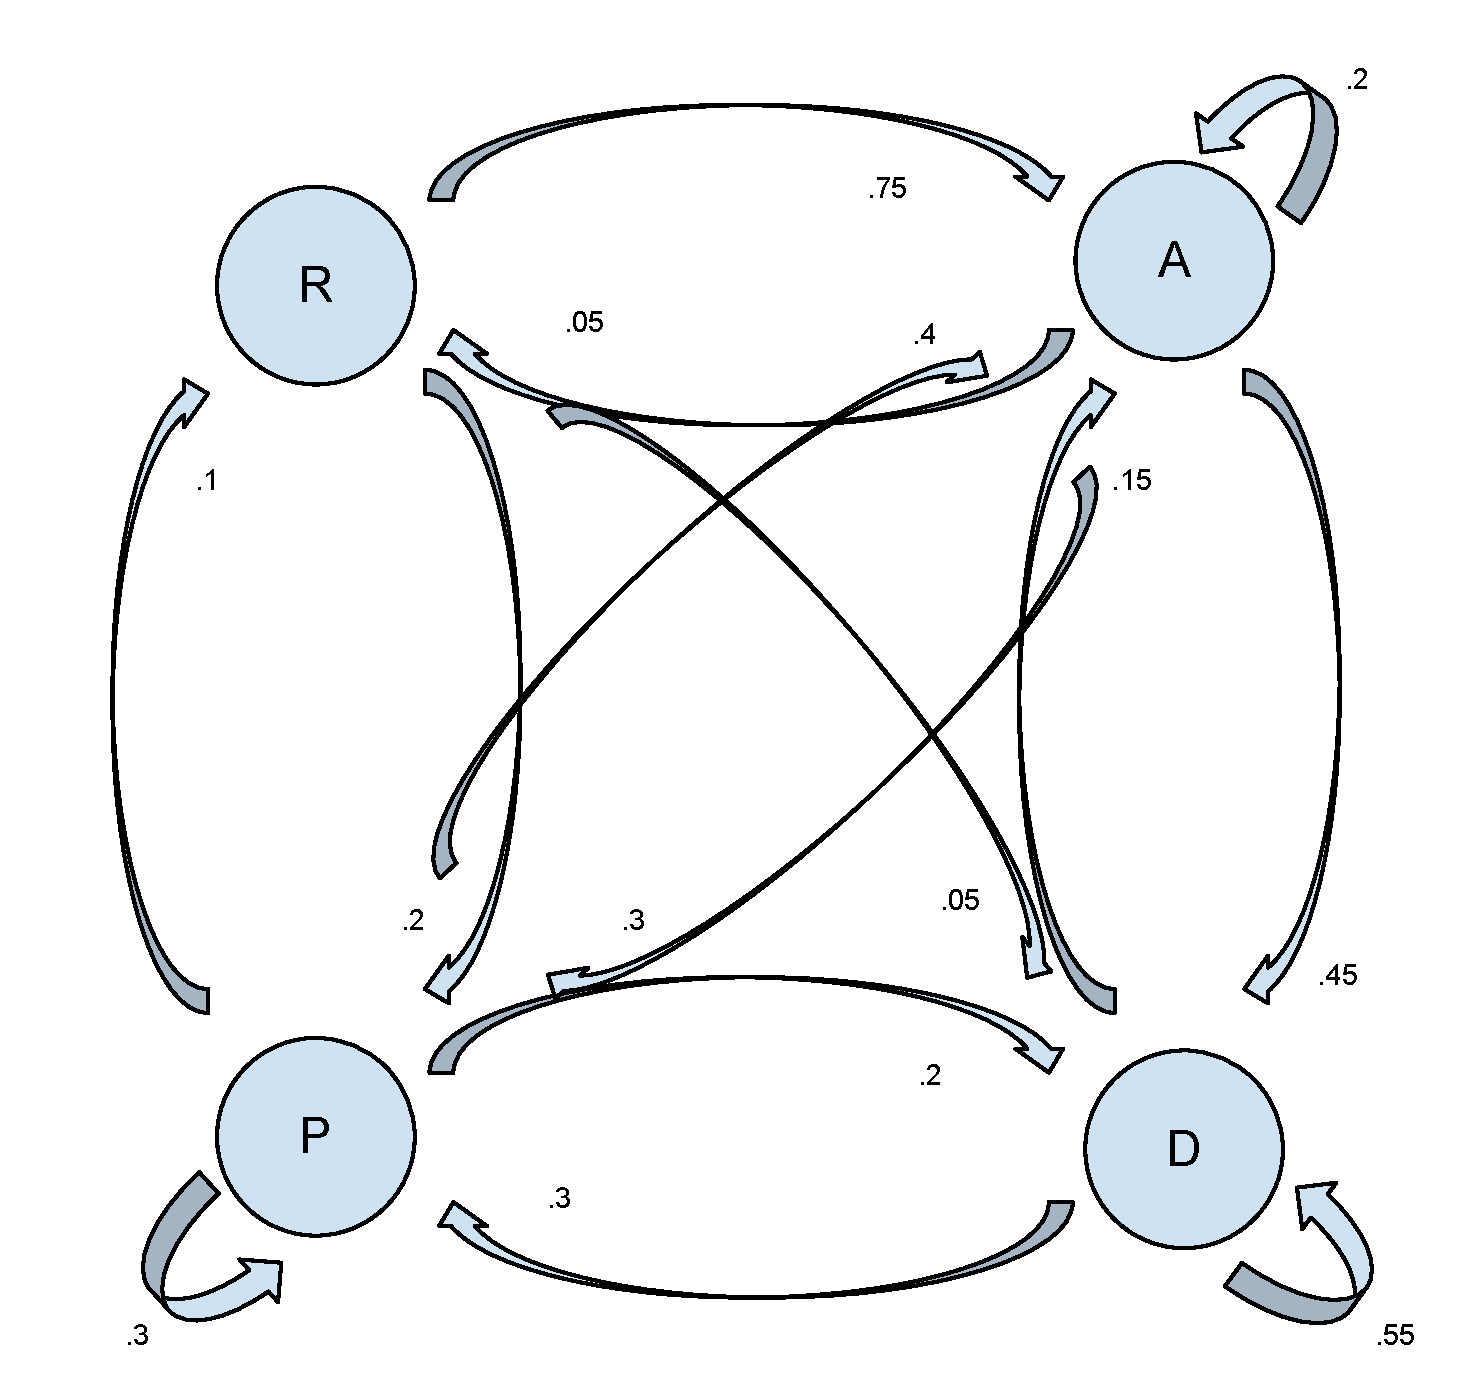
\includegraphics[width=8cm]{Markov_Chains_Ex_1.pdf}
\end{center}

$$
P=\begin{pmatrix}
0&.75&.2&.05\\
.05&.2&.3&.45\\
.1&.4&.3&.2\\
0&.15&.3&.55
\end{pmatrix}
$$

	\item Let us assume that a student starts their studies as ``Average''. What will be the probability of them being ``Rich'' after 1,2,3 time steps?

$$\pi^{(0)}=(0,1,0,0)$$


$$\pi^{(1)}=\pi^{(0)}P=(.05,.2,.3,.45)$$
After 1 time step: 5\% chance.
$$\pi^{(2)}=\pi^{(0)}P^2=(.04,.265,.295,.4)$$
After 2 time steps: 4\% chance.
$$\pi^{(3)}=\pi^{(0)}P^3=(.04275,.211,.296,.4025)$$
After 1 time step: 4.275\% chance.

	\item What is the steady state probability vector associated with this Markov chain?

The linear system:

$$
\begin{cases}
.05\pi_A+.1\pi_P&=\pi_R\\
.75\pi_R+.2\pi_A+.4\pi_P+.15\pi_D&=\pi_A\\
.2\pi_R+.3\pi_A+.3\pi_P+.3\pi_D&=\pi_P\\
.05\pi_R+.45\pi_A+.2\pi_P+.55\pi_D&=\pi_D\\
\pi_R+\pi_A+\pi_P+\pi_D=1
\end{cases}$$

has solution:
$$
\begin{cases}
\pi_R={53\over 1241}\\
\pi_A={326\over 1241}\\
\pi_P={367\over 1241}\\
\pi_D={495\over 1241}\\
\end{cases}$$


\end{enumerate}
\item Consider the following matrices. For the matrices that are stochastic matrices, draw the associated Markov Chain and obtain the steady state probabilities (if they exist, if not, explain why).


$$\begin{array}{cccc}
\begin{pmatrix}
0&1\\
0&1\\
\end{pmatrix}
&
\begin{pmatrix}
.5&.25&.25\\
1&0&0\\
0&.23&.77\\
.8&.1&.1
\end{pmatrix}&
\begin{pmatrix}
{1\over n}&{n-1\over n}\\
{n-1\over n}&{1\over n}\\
\end{pmatrix}
&
\begin{pmatrix}
.2&.3&.5\\
.1&.1&.8\\
.7&.1&.2
\end{pmatrix}\\
\text{(a)}&\text{(b)}& \text{(c)}&\text{(d)}\\
\begin{pmatrix}
.2&.3&.1&.4\\
0&.3&.7&0\\
.5&.2&.1&.2\\
.1&0&0&.9
\end{pmatrix}&
\begin{pmatrix}
.2&.3&.5\\
.3&-.3&1\\
.2&.2&.6
\end{pmatrix}
&
\begin{pmatrix}
.5&.5&0&0\\
0&.5&.5&0\\
0&0&.5&.5\\
.5&0&0&.5\\
\end{pmatrix}
&
\begin{pmatrix}
\alpha&\beta\\
\omega&\gamma
\end{pmatrix}
\\
\text{(e)}&\text{(f)}& \text{(g)}&\text{(h)}\\
\end{array}$$

\begin{enumerate}
\item
\begin{center}
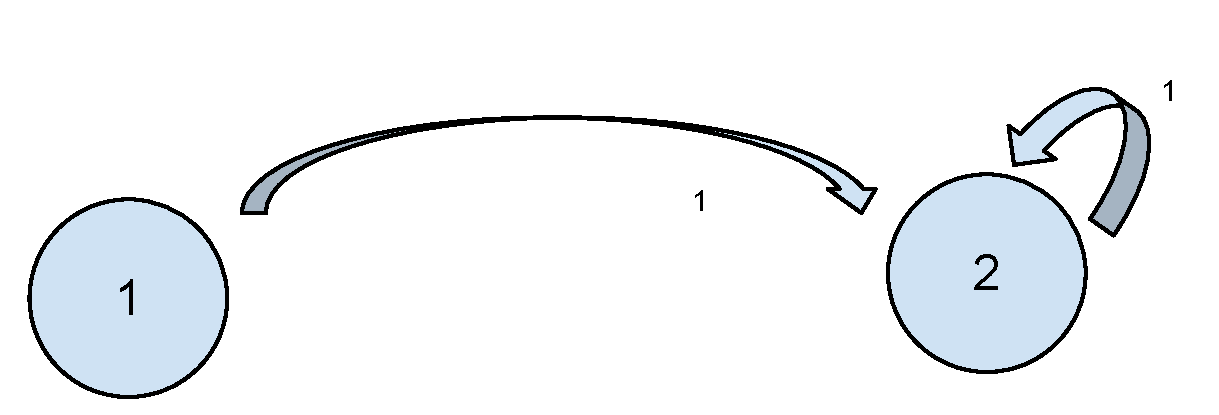
\includegraphics[width=8cm]{Markov_Chains_Ex_2-a.pdf}
\end{center}
$$\pi=(0,1)$$

\item Not a square matrix.
\item
For $0<n$:
\begin{center}
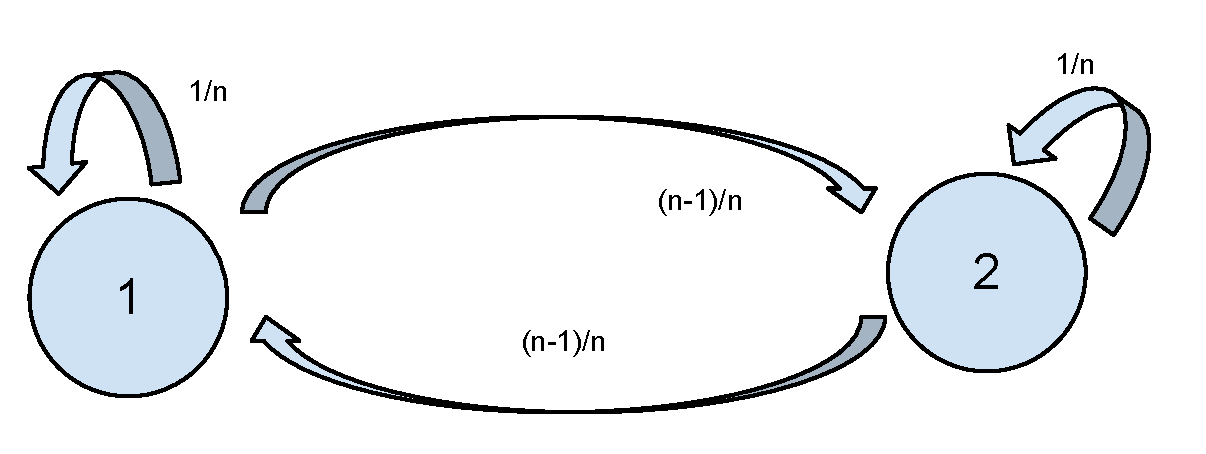
\includegraphics[width=8cm]{Markov_Chains_Ex_2-c.pdf}
\end{center}
$$\pi=(.5,.5)$$
\item
\begin{center}
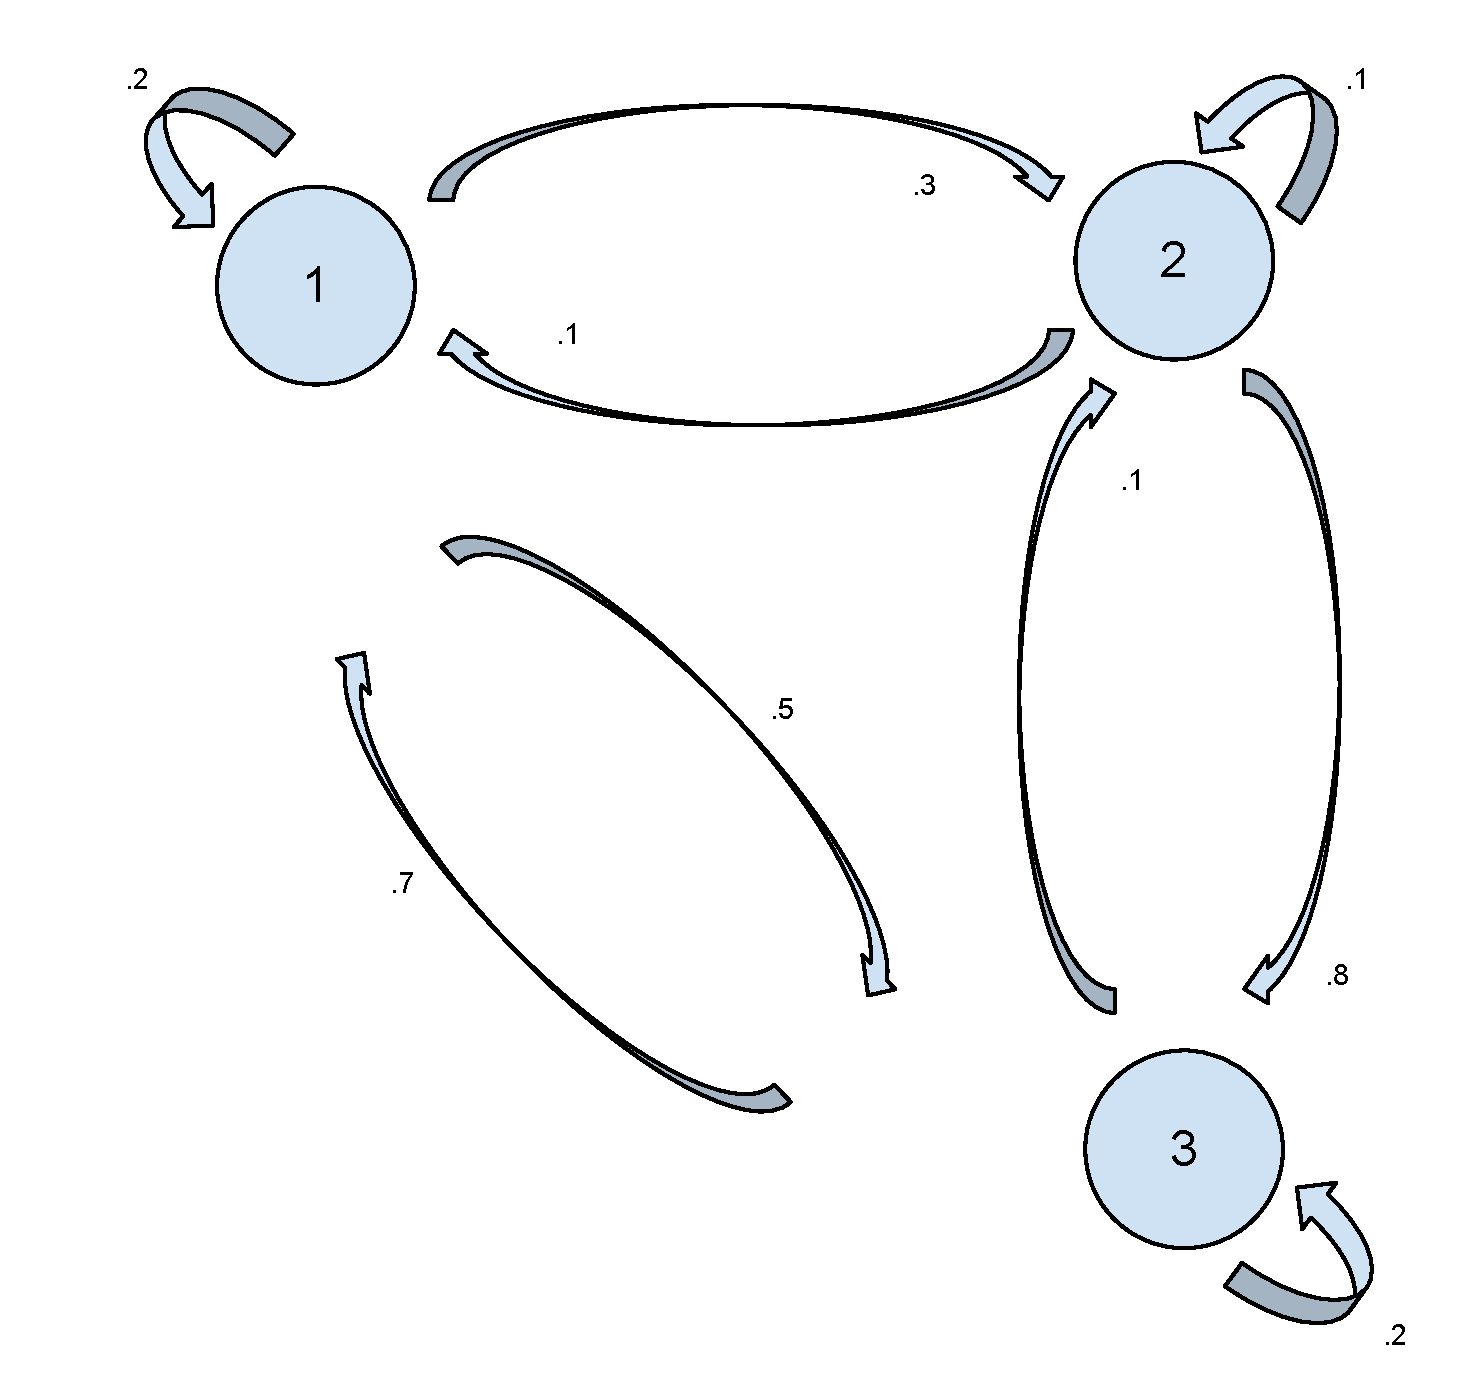
\includegraphics[width=8cm]{Markov_Chains_Ex_2-d.pdf}
\end{center}
$$\begin{cases}
.2\pi_1+.1\pi_2+.7\pi_3&=\pi_1\\
.3\pi_1+.1\pi_2+.1\pi_3&=\pi_2\\
.5\pi_1+.8\pi_2+.2\pi_3&=\pi_3\\
\pi_1+\pi_2+\pi_3&=1
\end{cases}$$
gives:
$$\pi=\left({32\over 81},{29\over 162},{23\over 54}\right)$$

\item
\begin{center}
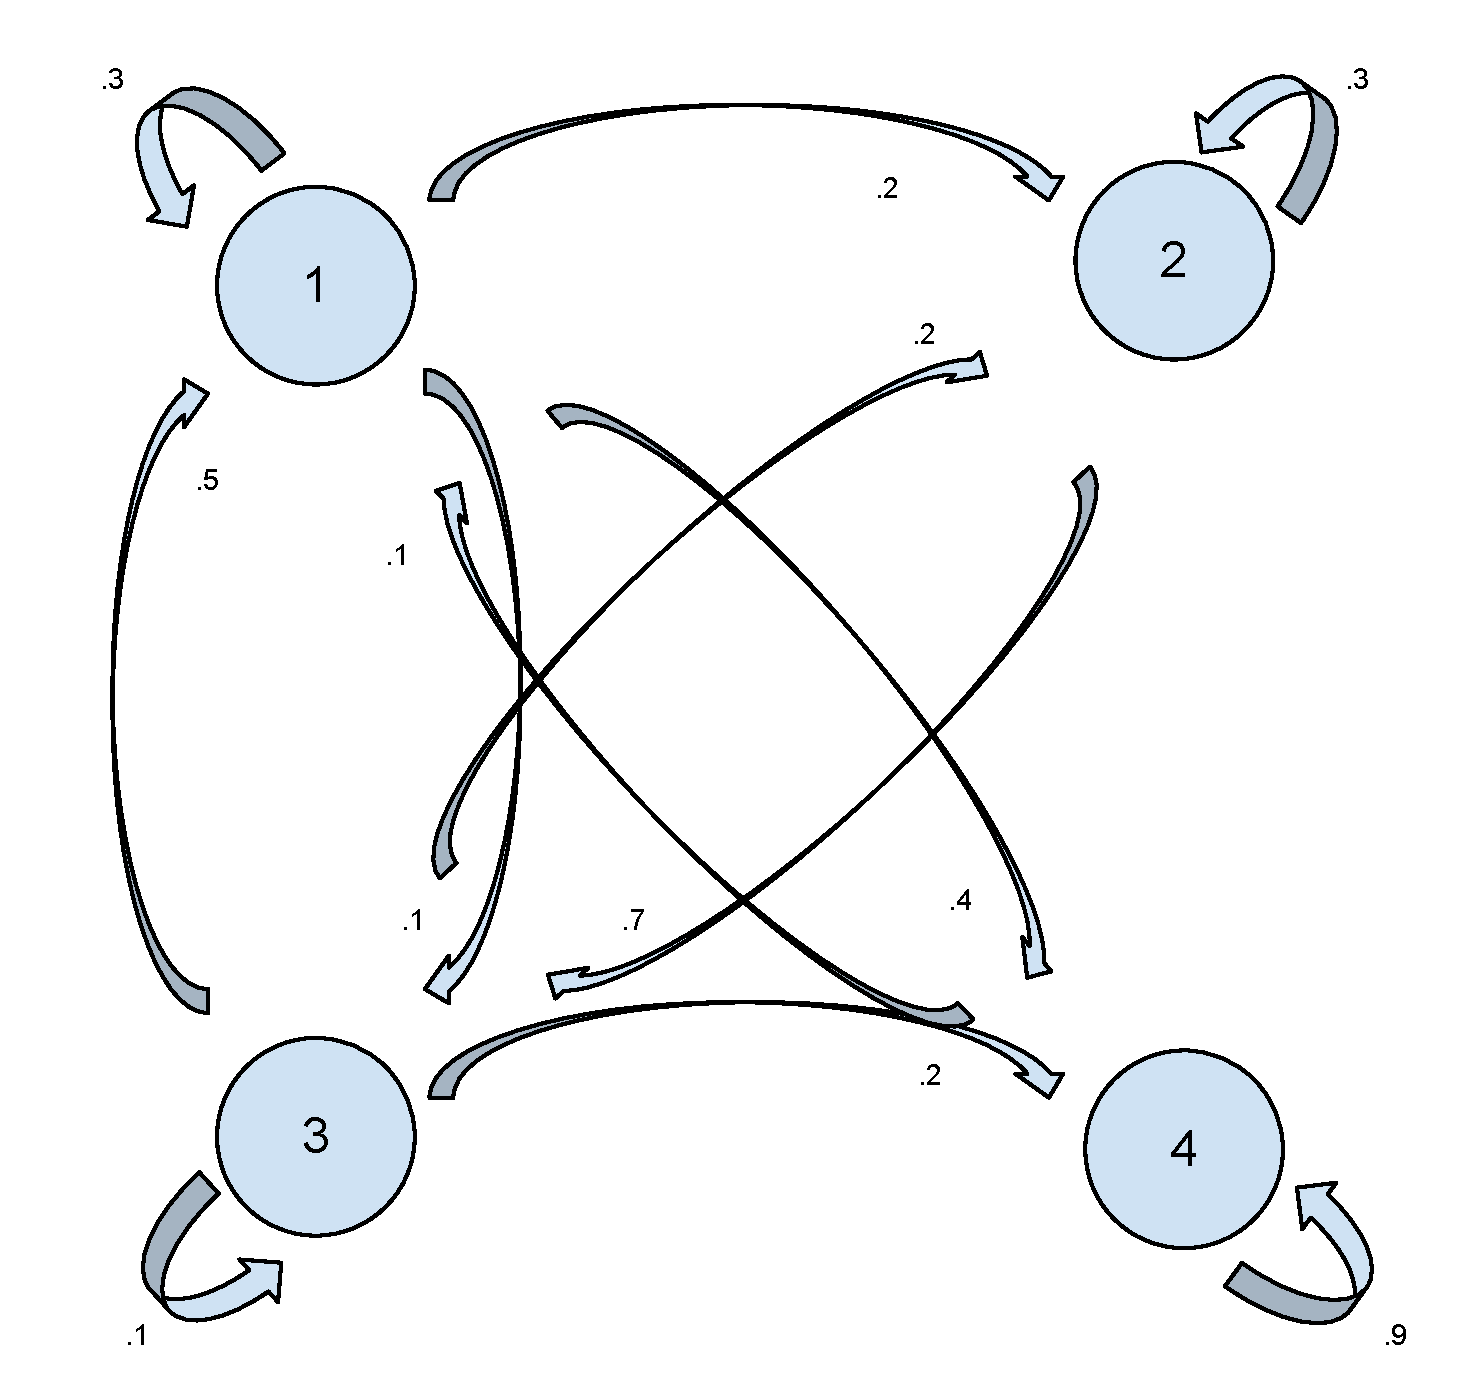
\includegraphics[width=8cm]{Markov_Chains_Ex_2-e.pdf}
\end{center}
$$
\begin{cases}
.2\pi_1+.5\pi_2+.1\pi_4&=\pi_1\\
.3\pi_1+.3\pi_2+.2\pi_3&=\pi_2\\
.1\pi_1+.7\pi_2+.1\pi_3&=\pi_3\\
.4\pi_1+.2\pi_3+.9\pi_4&=\pi_4\\
\pi_1+\pi_2+\pi_3+\pi_4&=1
\end{cases}$$

has solution:
$$
\pi=\left({49\over 358},{29\over 358},{14\over 179},{126\over 179}\right)
$$


\item $P_{22}<0$
\item

\begin{center}
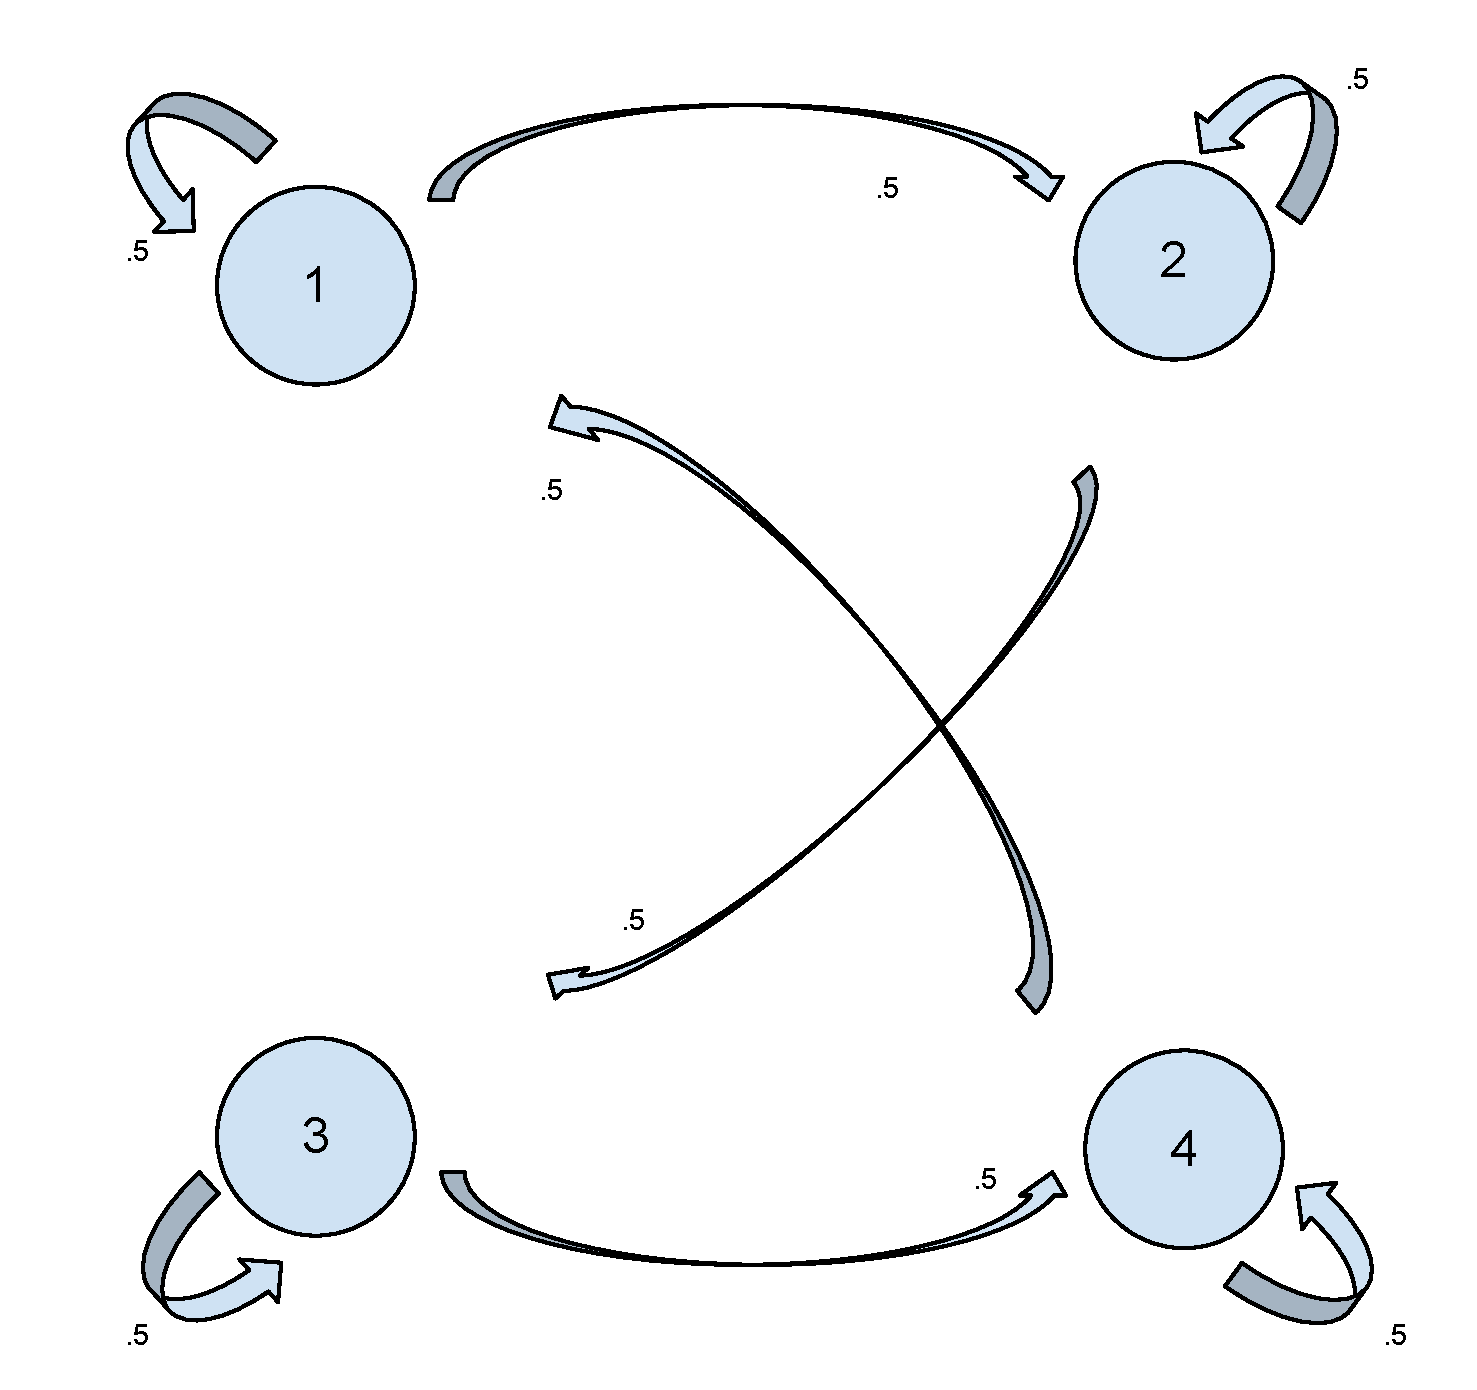
\includegraphics[width=8cm]{Markov_Chains_Ex_2-g.pdf}
\end{center}

Immediate to see that:

$$\pi=(.25,.25,.25,.25)$$

\item

Only if $\beta=1-\alpha>0$ and $\omega=1-\gamma>0$.

\end{enumerate}

\item Consider the following (incomplete) transition matrix:

$$
\begin{pmatrix}
?&2&1.5&.5\\
?&-5&1&3\\
5&2&?&1\\
1&?&1&-2\\
\end{pmatrix}
$$
\begin{enumerate}
	\item Fill in the missing values in the transition matrix.
$$
\begin{pmatrix}
-4&2&1.5&.5\\
1&-5&1&3\\
5&2&-8&1\\
1&0&1&-2\\
\end{pmatrix}
$$
	\item Draw the Markov chain.

\begin{center}
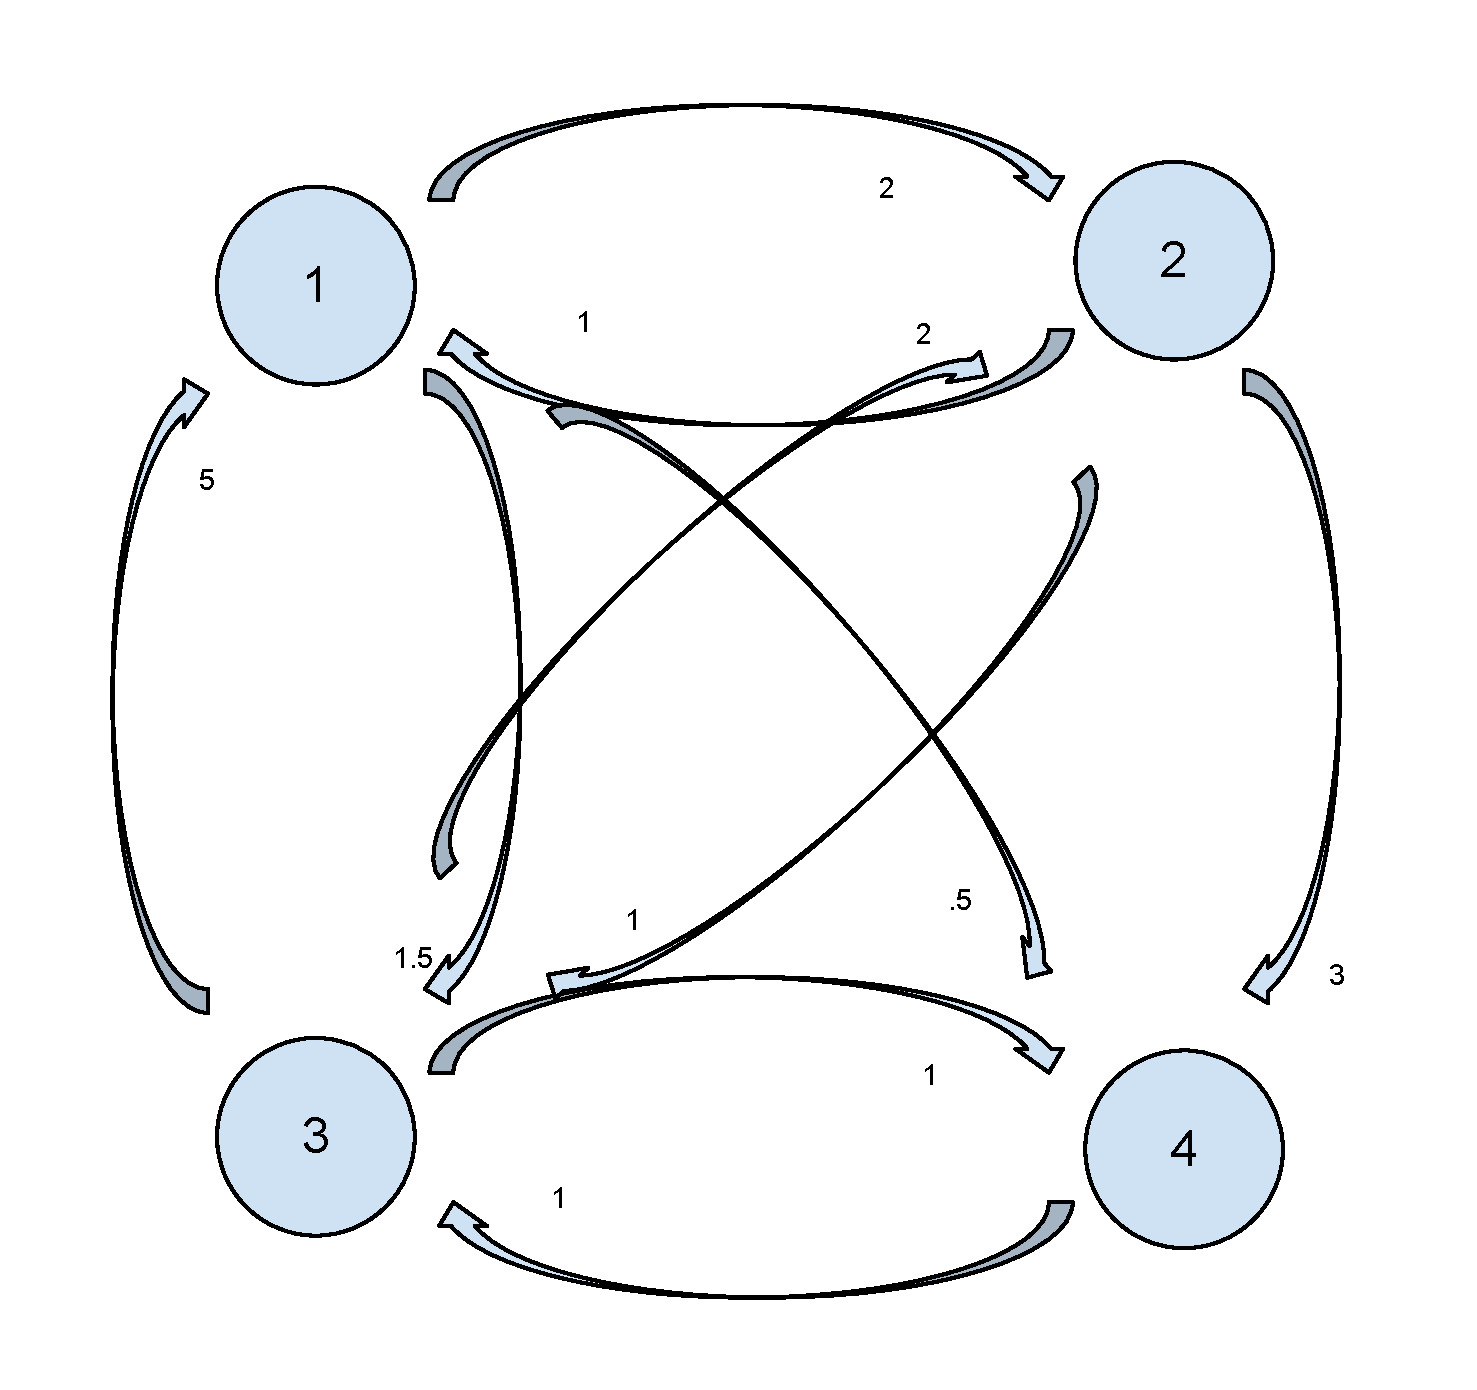
\includegraphics[width=8cm]{Markov_Chains_Ex_3.pdf}
\end{center}

	\item Obtain the steady state probabilities.
$$ \begin{cases}
-4\pi_1+\pi_2+5\pi_3+\pi_4&=0\\
2\pi_1-5\pi_2+2\pi_3&=0\\
1.5\pi_1+\pi_2-8\pi_3+\pi_4&=0\\
.5\pi_1+3\pi_2+\pi_3-2\pi_4&=0\\
\pi_1+\pi_2+\pi_3+\pi_4&=1
\end{cases}$$
has solution:

$$\pi=\left({13\over 43},{37\over 215},{11\over 86},{171\over 430}\right)$$

\end{enumerate}

\item Consider the following matrices. For the matrices that are transition rate matrices, draw the associated Markov Chain and obtain the steady state probabilities (if they exist, if not, explain why).

$$\begin{array}{cccc}
\begin{pmatrix}
-1&1\\
-1&1\\
\end{pmatrix}
&
\begin{pmatrix}
-5&0&5\\
2&0&-2\\
0&3&-3\\
0&0&0
\end{pmatrix}&
\begin{pmatrix}
-3&3&0\\
0&-3&3\\
3&0&-3
\end{pmatrix}
&
\begin{pmatrix}
-a&a&0\\
b&-(a+b)&a\\
0&b&-b
\end{pmatrix}\\
\text{(a)}&\text{(b)}& \text{(c)}&\text{(d)}\\
\begin{pmatrix}
-1&1&0&0\\
0&-4&2&2\\
1&0&-2&1\\
2&0&0&-2
\end{pmatrix}&
\begin{pmatrix}
0&0&0\\
5&-10&5\\
10&0&-10
\end{pmatrix}
&
\begin{pmatrix}
-.5&.5&0&0\\
0&-.5&.5&0\\
0&0&-.5&.5\\
.5&0&0&-.5\\
\end{pmatrix}
&
\begin{pmatrix}
\alpha&\beta\\
\omega&\gamma
\end{pmatrix}
\\
\text{(e)}&\text{(f)}& \text{(g)}&\text{(h)}\\
\end{array}$$

\begin{enumerate}
\item $P_{22}>0$
\item Not a square matrix.
\item
\begin{center}
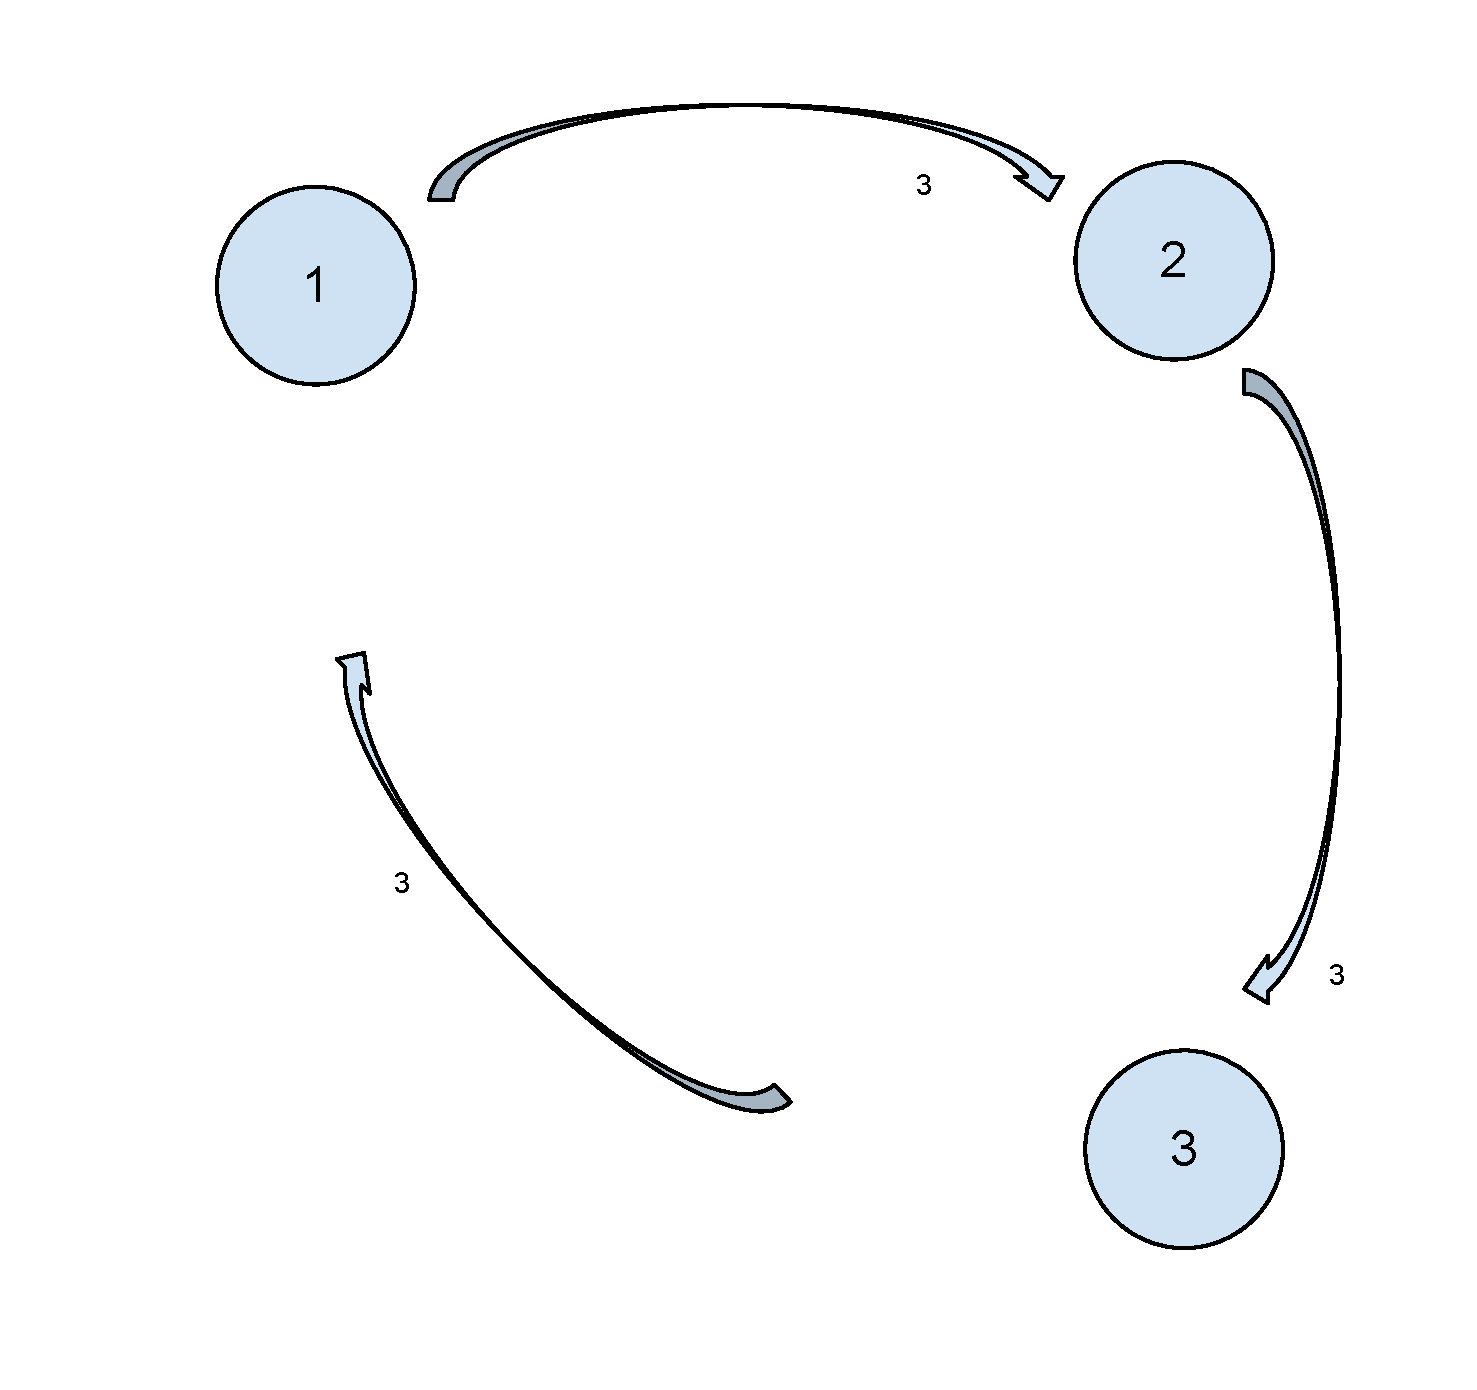
\includegraphics[width=8cm]{Markov_Chains_Ex_4-c.pdf}
\end{center}
$$\pi=\left({1\over3},{1\over3},{1\over3}\right)$$


\item
\begin{center}
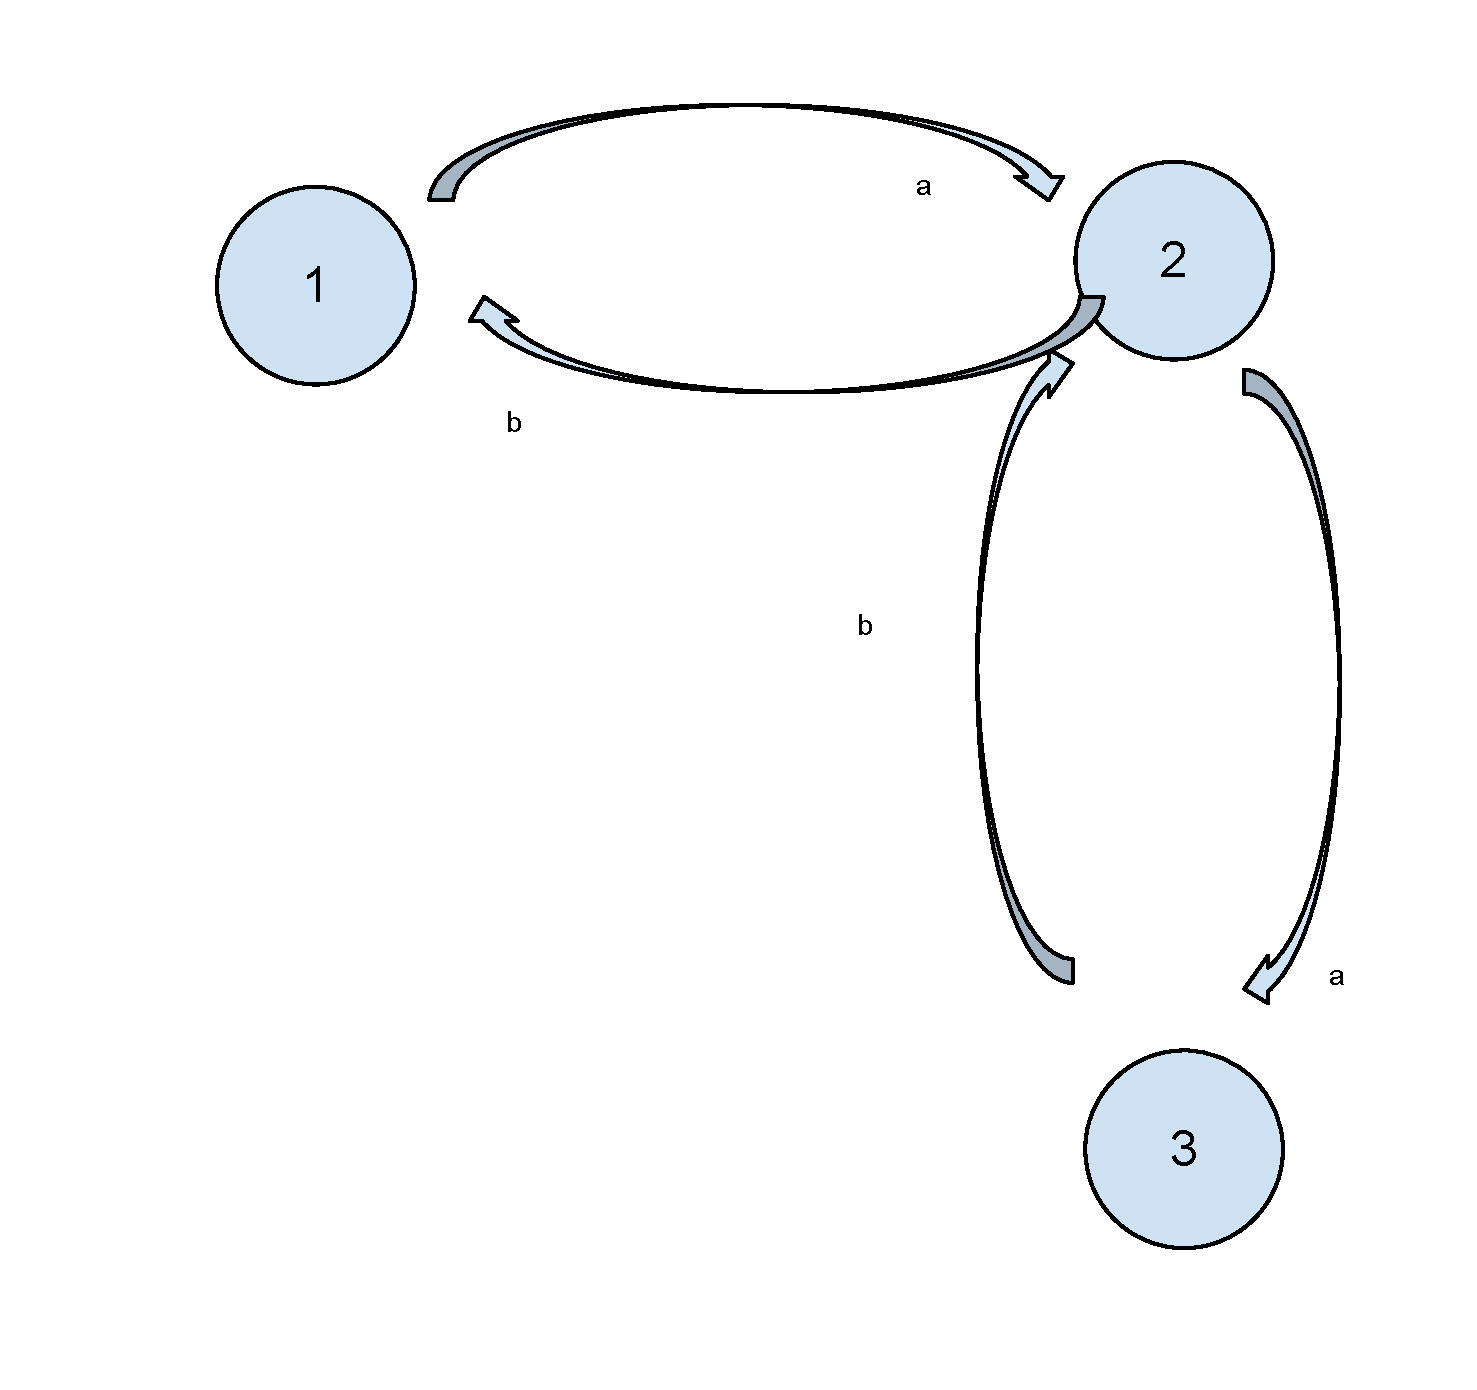
\includegraphics[width=8cm]{Markov_Chains_Ex_4-d.pdf}
\end{center}
$$ \begin{cases}
-a\pi_1+a\pi_2&=0\Rightarrow\pi_1=\pi_2\\
b\pi_1-(a+b)\pi_2+a\pi_3&=0\Rightarrow\pi_2=\pi_3\\
b\pi_2-b\pi_3&=0\Rightarrow\pi_2=\pi_3\\
\pi_1+\pi_2+\pi_3=1
\end{cases}
$$
thus:
$$\pi=\left({1\over3},{1\over3},{1\over3}\right)$$

\item

\begin{center}
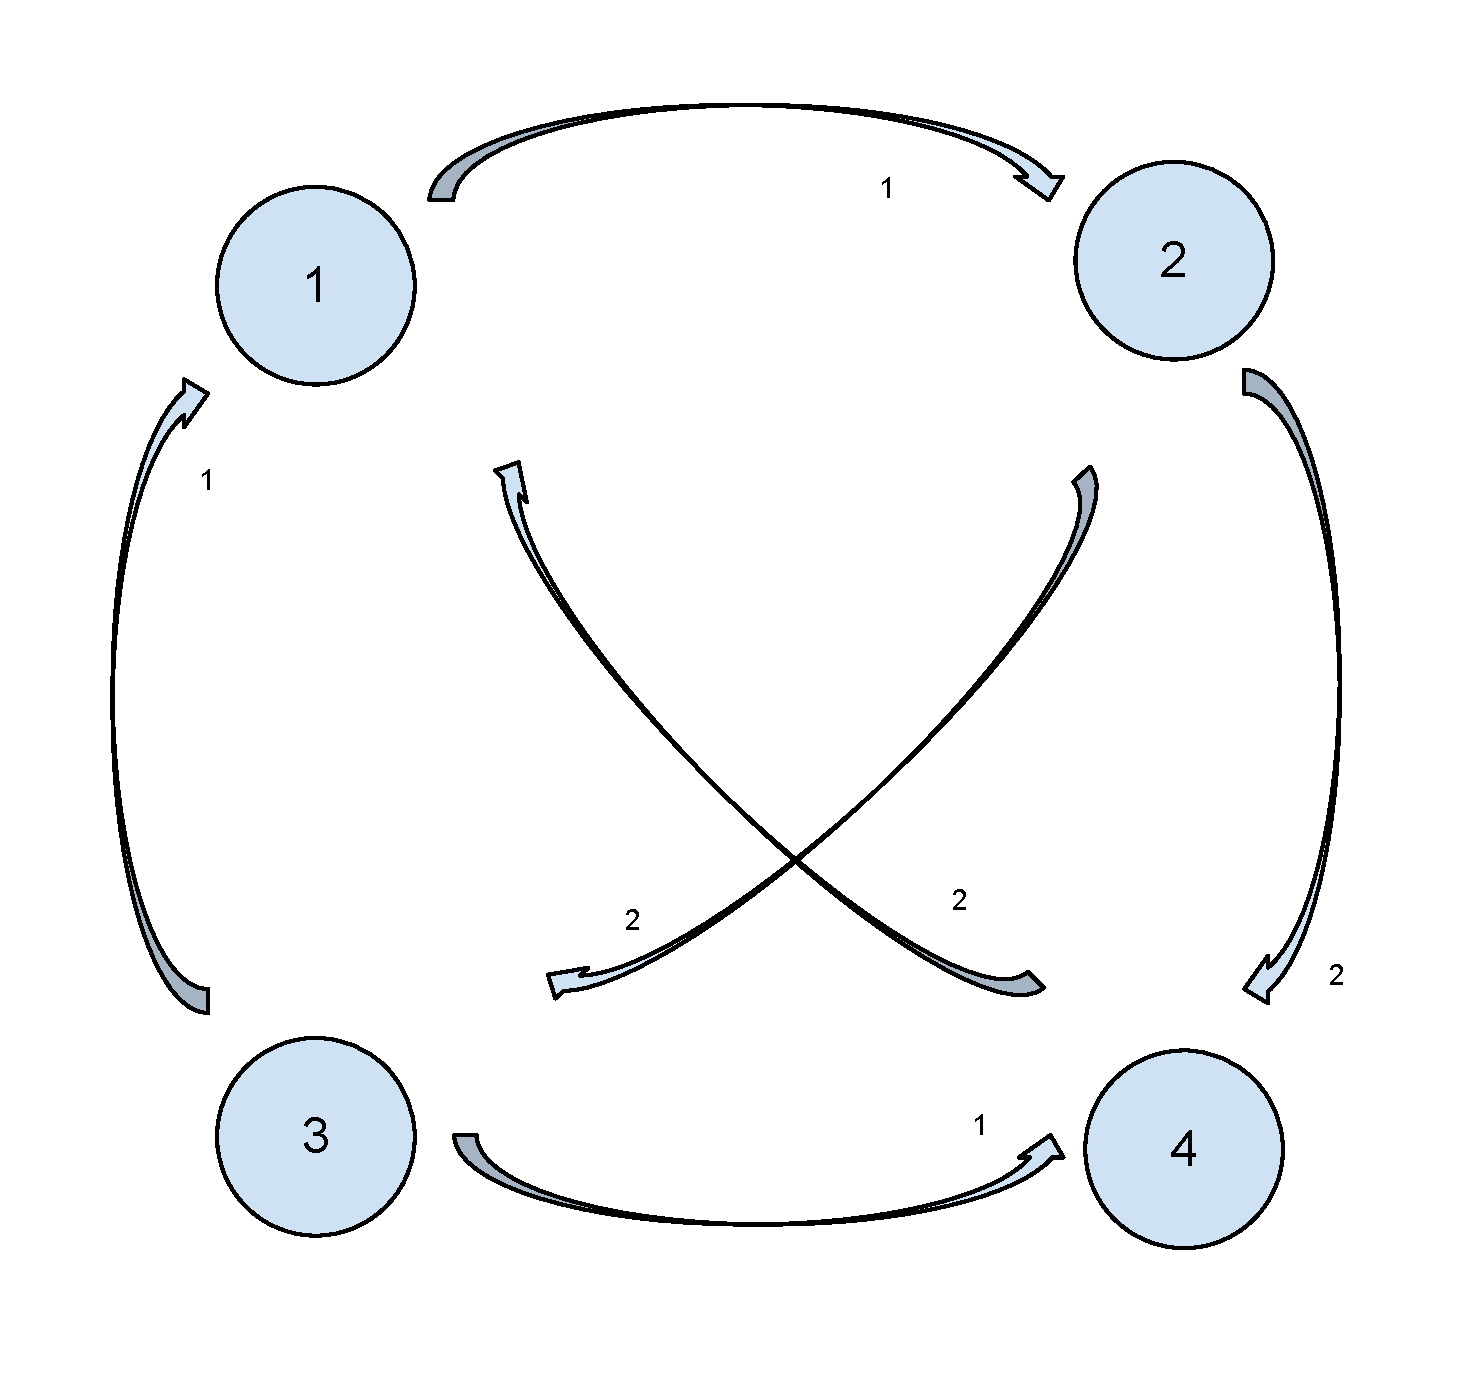
\includegraphics[width=8cm]{Markov_Chains_Ex_4-e.pdf}
\end{center}


$$ \begin{cases}
-\pi_1+\pi_3+2\pi_4&=0\\
\pi_1-4\pi_2&=0\\
2\pi_2-2\pi_3&=0\\
2\pi_2+\pi_3-2\pi_4&=0\\
\pi_1+\pi_2+\pi_3+\pi_4&=1
\end{cases}$$
gives:
$$\pi=\left({8\over15},{2\over15},{2\over15},{3\over15}\right)$$

\item

\begin{center}
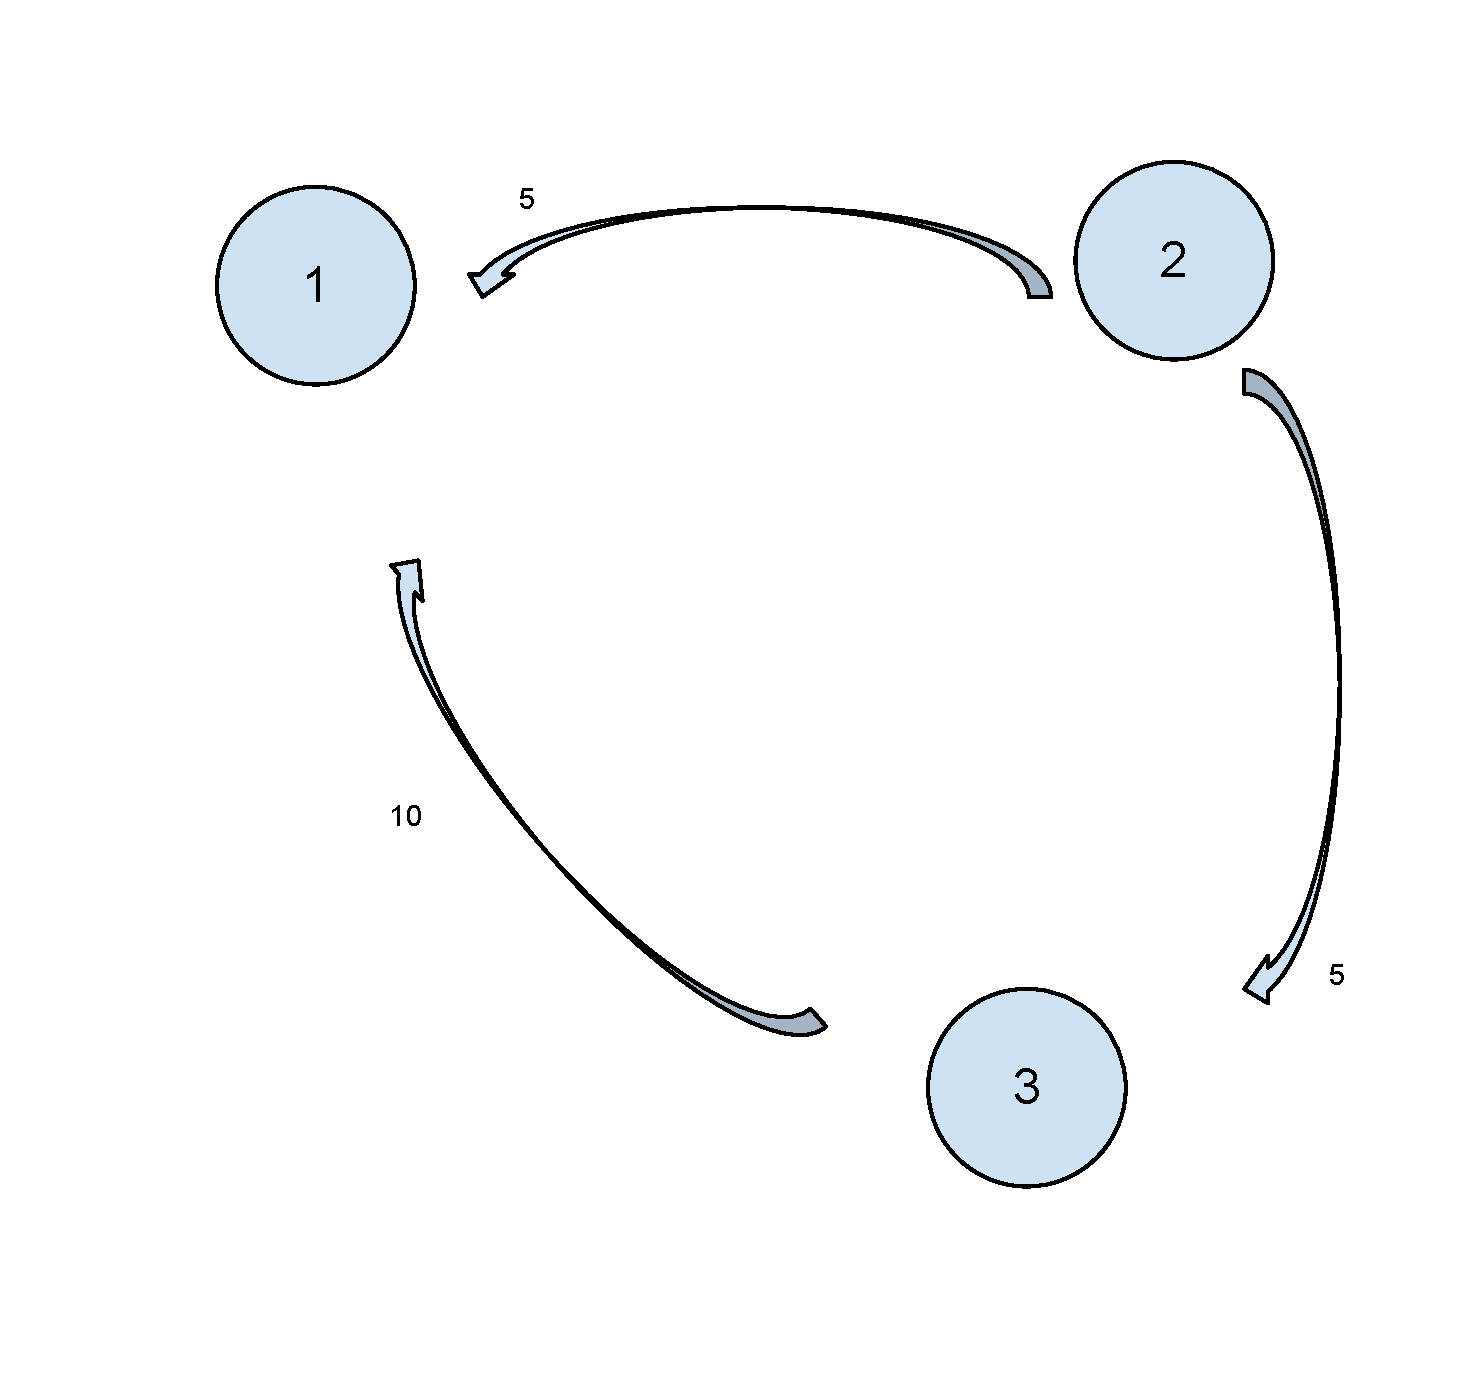
\includegraphics[width=8cm]{Markov_Chains_Ex_4-f.pdf}
\end{center}

$$\pi=(1,0,0)$$

\item
\begin{center}
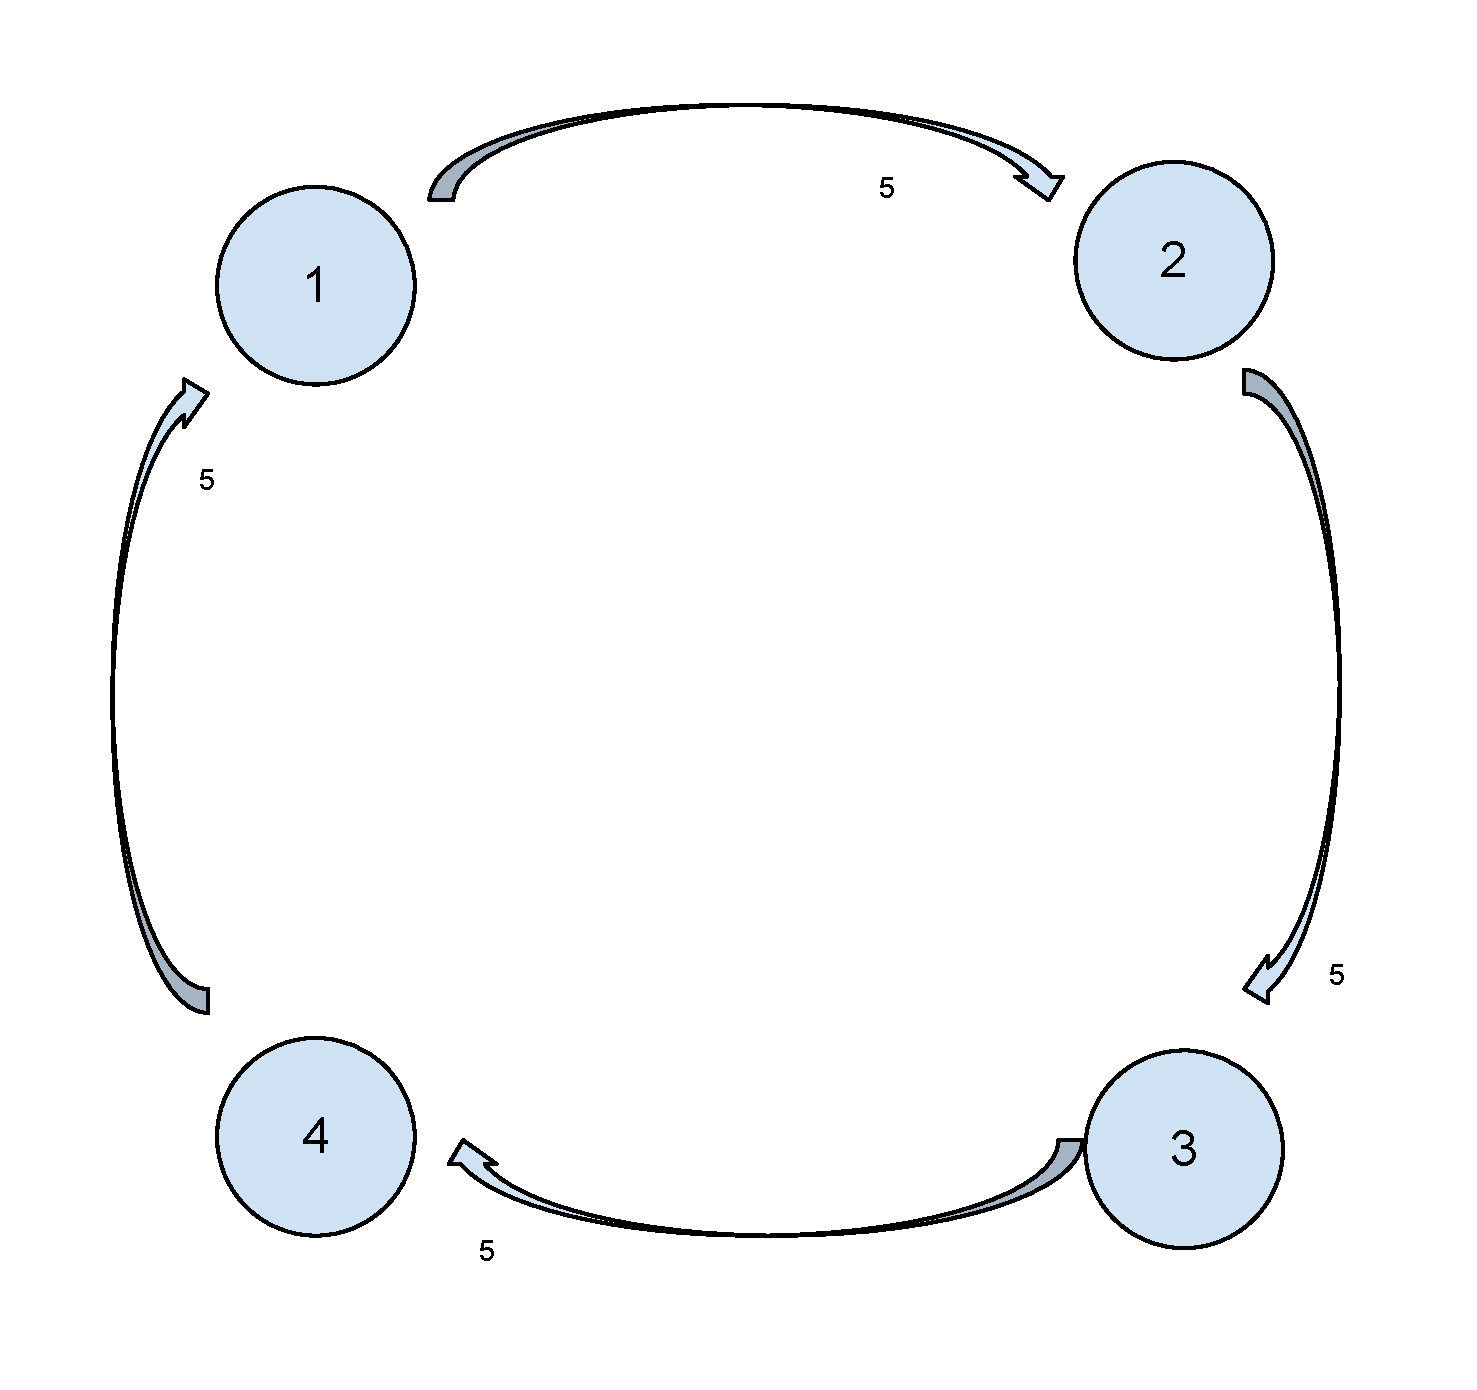
\includegraphics[width=8cm]{Markov_Chains_Ex_4-g.pdf}
\end{center}

$$\pi=\left({1\over4},{1\over 4},{1\over 4},{1\over 4}\right)$$

\item Only if $-\alpha=\beta\geq0$ and $-\gamma=\omega\geq0$


\begin{center}
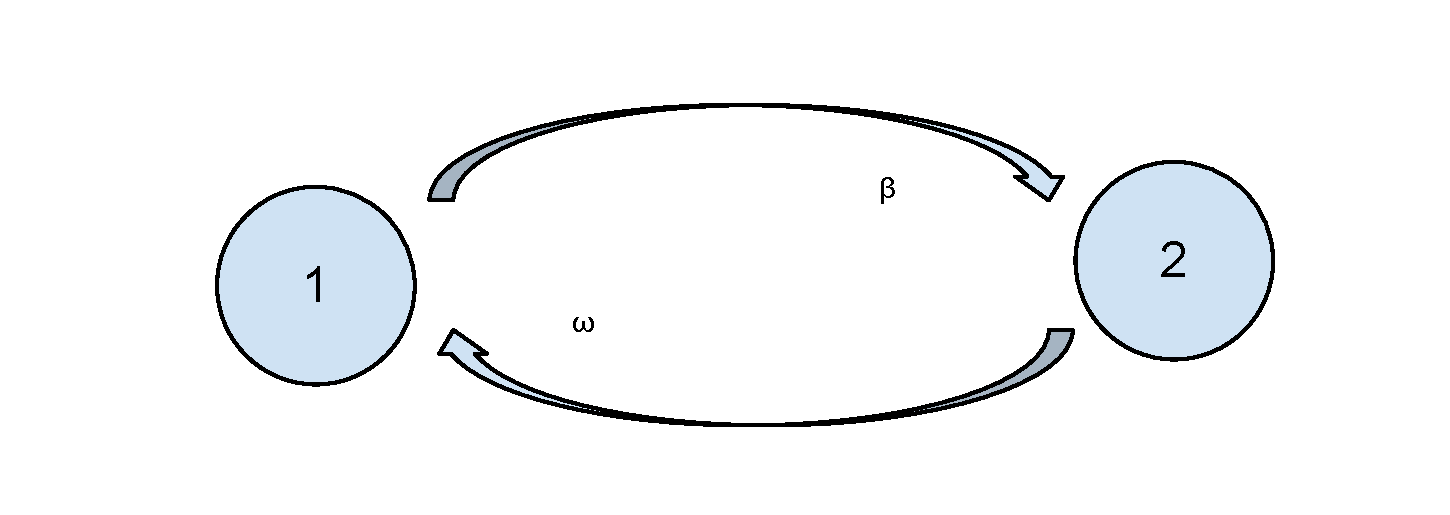
\includegraphics[width=8cm]{Markov_Chains_Ex_4-h.pdf}
\end{center}

$$\begin{cases}
-\beta\pi_1+\omega\pi_2&=0\\
\pi_1+\pi_2=1
\end{cases}$$
Gives:
$$\pi=\left({\omega\over \beta+\omega},{\beta\over\beta+\omega}\right)$$
if $\beta+\omega=0$ then no steady state exists.

\end{enumerate}
\item Consider the following continuous Markov chain.

\begin{center}
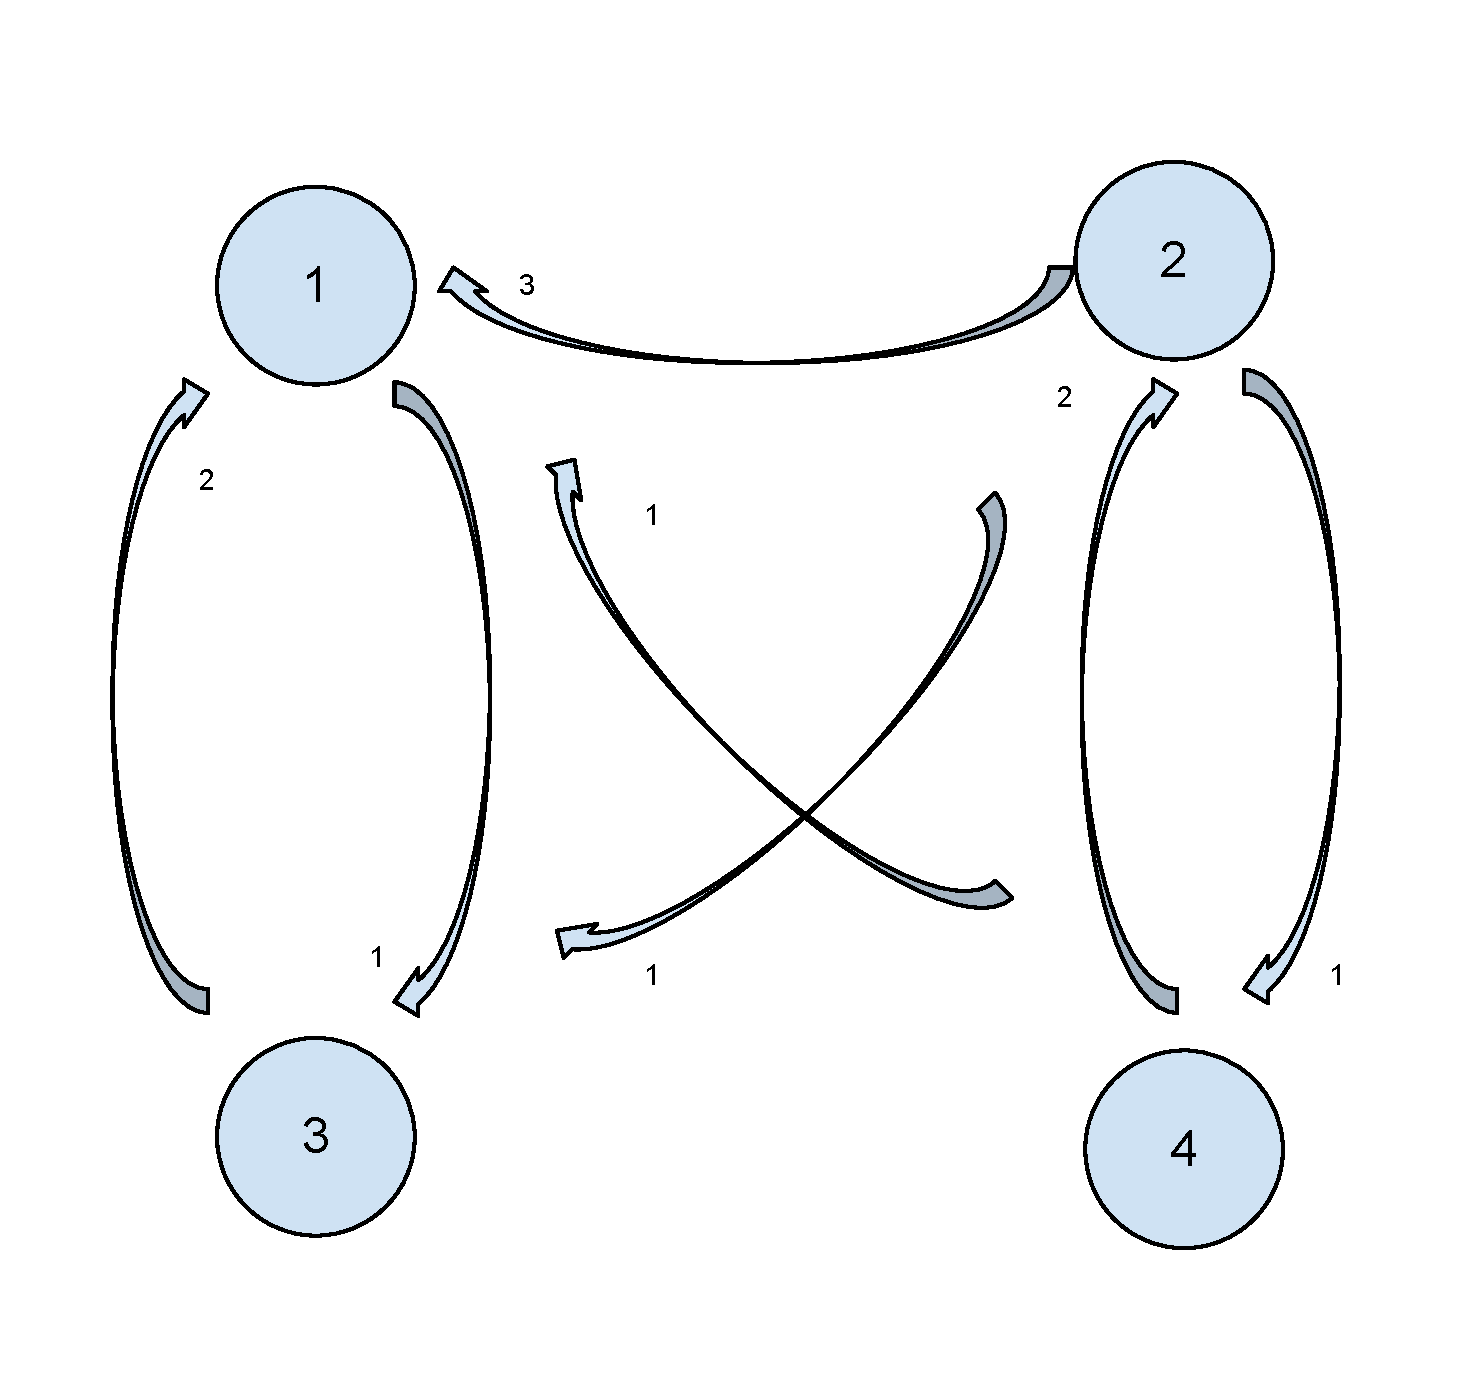
\includegraphics[width=8cm]{Markov_Chains_Ex_5.pdf}
\end{center}



\begin{enumerate}
	\item Obtain the transition rate matrix.
$$Q=\begin{pmatrix}
-1&0&1&0\\
3&-5&1&1\\
2&0&-2&0\\
1&2&0&-3\\
\end{pmatrix}$$

	\item Obtain the steady state probabilities for this Markov chain.
$$
\begin{cases}
-\pi_1+3\pi_2+2\pi_3+\pi_4&=0\\
-5\pi_2+2\pi_4&=0\\
\pi_1+\pi_2-2\pi_3&=0\\
\pi_2-3\pi_4&=0
\end{cases}
$$
has solution:
$$\left({2\over3},0,{1\over3},0\right)$$

	\item Obtain the corresponding discrete time Markov chain.

Taking $\Delta t={1\over 5}$ gives:

$$P=\begin{pmatrix}
{4\over5}&0&{1\over5}&0\\
{3\over5}&0&{1\over5}&{1\over5}\\
{2\over 5}&0&{3\over5}&0\\
{1\over 5}&{2\over5}&0&{2\over 5}\\
\end{pmatrix}$$


	\item Draw the corresponding Markov chain.

\begin{center}
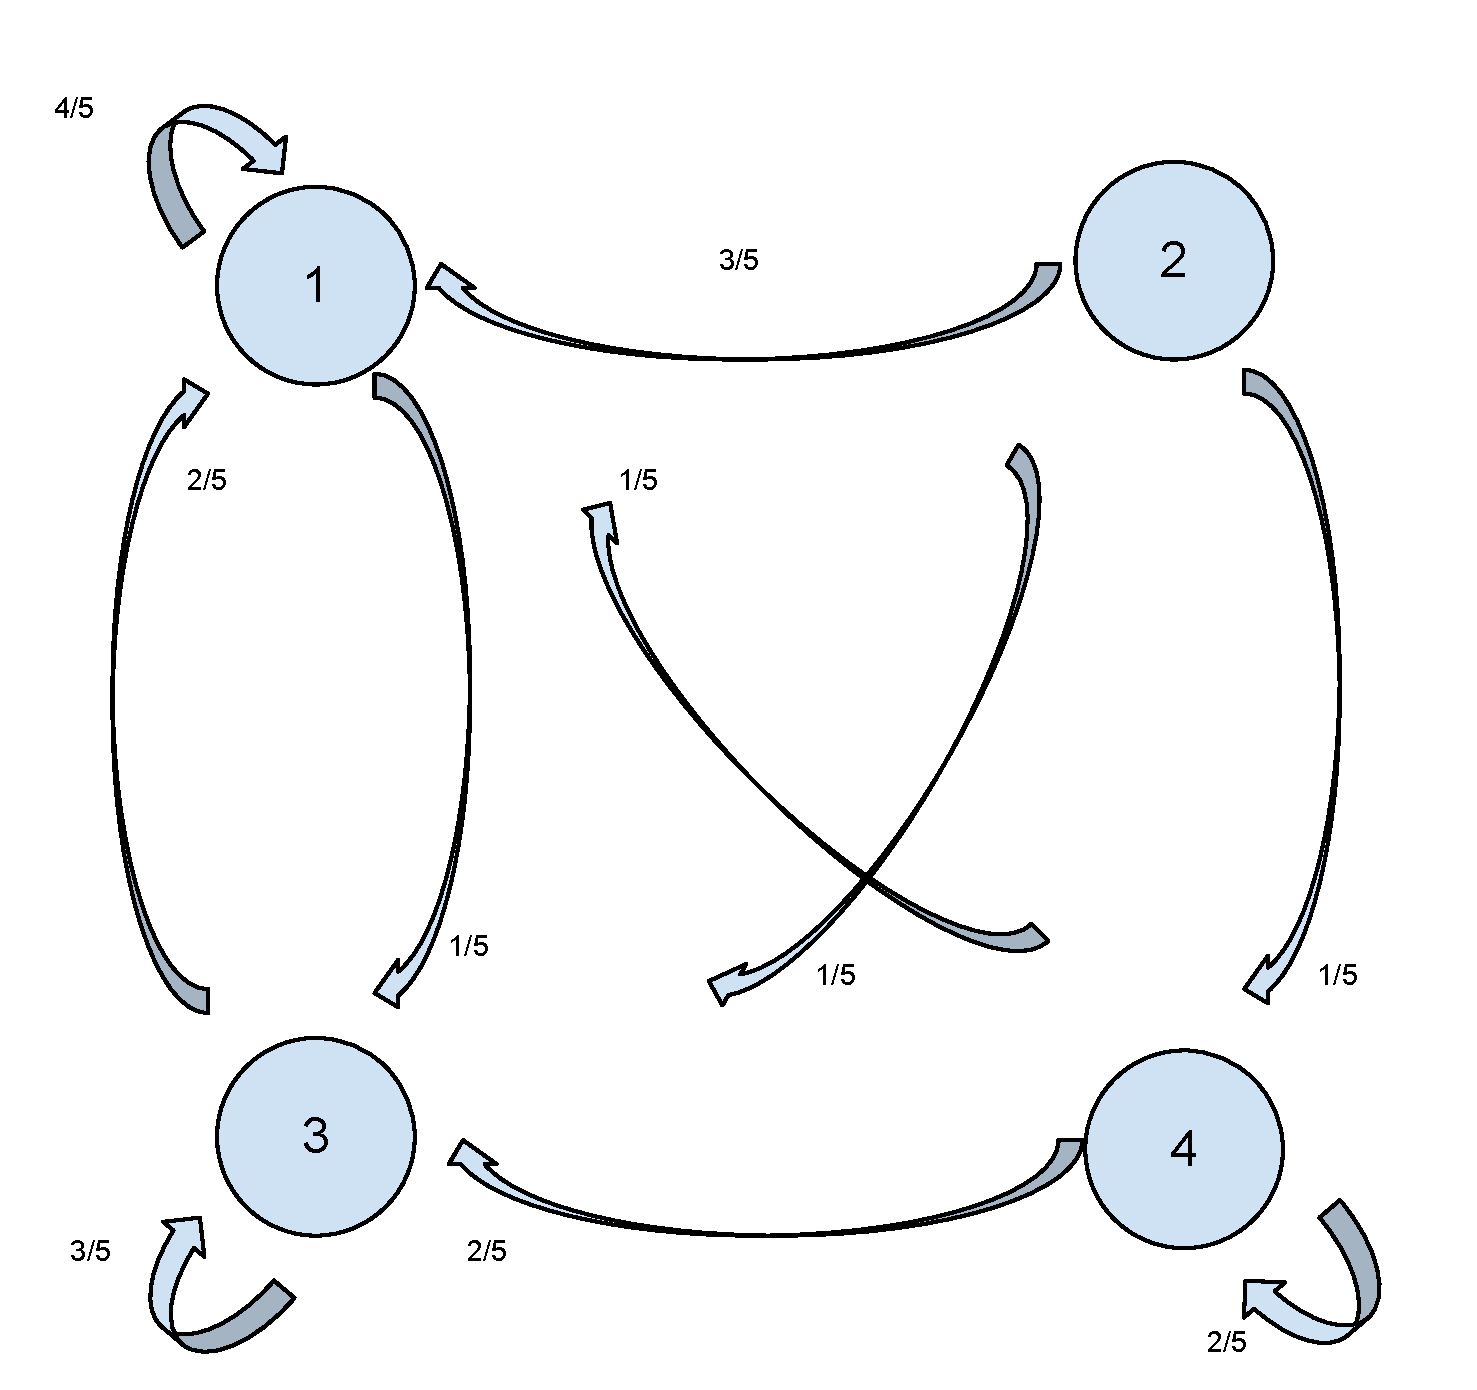
\includegraphics[width=8cm]{Markov_Chains_Ex_5-d.pdf}
\end{center}

	\item Obtain the steady state probabilities for the discretized Markov chain.
$$
\begin{cases}
{4\over5}\pi_1+{3\over5}\pi_2+{2\over5}\pi_3+{1\over5}\pi_4&=\pi_1\\
{2\over5}\pi_4&=\pi_2\\
{1\over5}\pi_1+{1\over5}\pi_2+{3\over5}\pi_3&=\pi_3\\
{1\over5}\pi_2+{2\over5}\pi_4&=\pi_4\\
\pi_1+\pi_2+\pi_3+\pi_4&=1
\end{cases}
$$
has solution:
$$\left({2\over3},0,{1\over3},0\right)$$
\end{enumerate}

\end{enumerate}

\end{document}
